%\review


\chapter{Конформная теория поля и аффинные алгебры Ли}
\label{cha:CFT}

Двумерная конформная теория поля возникла в результате обобщения гипотезы о масштабной инвариантности критического поведения в двумерных системах \cite{Polyakov:1970xd}. Если использовать теорию поля для описания критического поведения, то такая теория должна обладать конформной инвариантностью. 

Глобальная конформная инвариантность в произвольном числе измерений ведет к важным физическим следствиям. Например, особый интерес в последнее время привлекла $N=4$ суперсимметричная модель Янга-Миллса.

 Однако в случае двумерной теории важнейшую роль играет локальная конформная инвариантность.  Такая теория обладает богатой симметрией, так что ее даже иногда называют точно решаемой \cite{belavin1984ics}.

Конформное преобразование --- это преобразование, меняющее только масштаб у метрического тензора:
\begin{equation}
  \label{eq:10}
  g'_{\mu\nu}(x')=\Lambda(x)g_{\mu\nu}(x)
\end{equation}
На двумерной мировой поверхности удобно ввести комплексные координаты $z,\bar{z}$. 
В двумерном случае существует бесконечное число локально-конформных преобразований $z\to w(z)$.
Это легко видеть из условия конформности преобразований, так как в двумерном случае такое
условие эквивалентно уравнению Коши-Римана для голоморфных функций ($\partial_{\bar z}w(z,\bar
z)=0$).

Таким образом, локально-конформные преобразования находятся в однозначном соответствии с множеством
всех аналитических функций $w(z)$ на плоскости.  

Глобальные конформные преобразования имеют вид
\begin{equation}
  \label{eq:172}
  w(z)=\frac{az+b}{cz+d},\; ad-bc=1ю
\end{equation}


Рассмотрим инфинитезимальные преобразования $w(z)=z+\epsilon(z),\quad \epsilon(z)=\sum_{-\infty}^{\infty}c_nz^{n+1}$. 
Тогда для бесспинового поля $\phi(z,\bar z)$ верно следующее: $\phi'(z',\bar z')=\phi(z,\bar z)$,
$\delta\phi=-\epsilon(z)\partial\phi-\bar \epsilon(\bar z)\bar \partial \phi=\sum_n(c_n L_n\phi+\bar
c_n\bar L_n\phi)$, где $L_n=-z^{n+1}\partial_z,\quad \bar L_n=-\bar z^{n+1}\partial_{\bar z}$

Мы видим, что в классической теории алгебра конформных преобразований --- это алгебра Витта, которая
порождается генераторами $\{L_n, n\in \mathbb{Z}\}$ --- модами разложения оператора энергии-импульса $T$, с
коммутационными соотношениями
\begin{equation}
  \label{eq:2}
  [L_m,L_n]=(m-n)L_{m+n}
\end{equation}
При квантовании возникает конформная аномалия, что соответствует центральному расширению \eqref{eq:62} алгебры  (то
есть появлению центрального заряда $c$). В коммутационные соотношения надо добавить член
$\frac{c}{12}(m^3-m)\delta_{m+n,0}$. В результате получаем алгебру Вирасоро.

Поля теории $\phi(z,\bar z)$ должны преобразовываться определенным образом при конформных преобразованиях.
Оказывается, что все поля группируются в конформные семейства, в которых есть одно примарное поле
\begin{equation}
  \label{eq:3}
  \begin{split}
    \phi_{h,\bar h}(z,\bar z)\underset{
      \genfrac{}{}{0pt}{}{z\to w(z)}
        {\bar z \to \bar w(\bar z)}
    }
    {\longrightarrow} \left(\frac{dw}{dz}\right)^{h}\left(\frac{d\bar w}{d\bar
        z}\right)^{\bar h}\phi_{h,\bar h}(w(z),\bar w(\bar z))\\
    L_n \phi=0,\quad n>0\\
    L_0 \phi=h \phi\\
  \end{split}
\end{equation}
$h, \bar h$ называются конформными весами поля.
Все остальные поля называются вторичными и получаются из примарного действием операторов $L_{-n}$:
\begin{equation}
  \label{eq:67}
  L_{-n_1}L_{-n_2}\dots \phi_{h,\bar h}
\end{equation}
Все поля в теории оказываются суммами произведений элементов мультиплетов алгебры Вирасоро.

Алгебраические методы позволяют получать огромное количество точных результатов в двумерных конформных теориях поля. Существуют разнообразные классы моделей двумерной конформной теории поля и даже задача классификации всех таких моделей до конца не решена, несмотря на первоначальный оптимизм \cite{moore1989taming}.  Помимо описания критических явлений, конформная теория поля привлекла большое внимание благодаря своей связи с теорией струн.

Двумерная конформная теория поля выделяется как модель квантовой теории поля из-за того, что она может быть сформулирована аксиоматически. В данной главе мы приводим такую аксиоматическую формулировку в разделе \ref{sec:conformal-field-theory-general}, а затем рассматриваем важнейшие классы моделей конформной теории -- модели Весса-Зумино-Новикова-Виттена \ref{sec:WZNW-models} и coset-модели \ref{sec:coset-models-cft}. Эти модели обладают дополнительными симметриями, выражающимися на языке теории представлений аффинных алгебр Ли и являются естественным приложением математических результатов данной диссертации. 

В том случае, если в теории конечное число примарных полей, такая теория называется минимальной.  Обычно соответствие между критическим поведением решеточных моделей и конформной теорией поля устанавливается именно для минимальных моделей \cite{belavin1984ics}.  

Строгое доказательство соответствия между критическим поведением решеточных моделей и конформной теории поля остается серьезной проблемой, но  в последнее время получены новые результаты, связанные с использованием  эволюции Шрамма-Лёвнера. Этот подход основывается на сопоставлении доменных стенок в решеточных моделях с траекториями случайного процесса, называющегося эволюцией Шрамма-Лёвнера \cite{schramm2000scaling}. Для простых моделей, типа модели Изинга, удается доказать, что некоторая наблюдаемая --  мартингал по отношению к эволюции Шрамма-Лёвнера, -- обладает конформной инвариантностью. Оказывается, что этого достаточно для доказательства конформной инвариантности критического поведения модели \cite{duminil2011conformal}. Такая техника сильно отличается от теоретико-полевого описания, поэтому актуальна проблема установления соответствия между эволюцией Шрамма-Лёвнера и конформной теорией поля \cite{bauer2002sle,bauer2003conformal,bauer2003sle,bauer2004cfts,bauer2004sle,bauer2004conformal}. 

В главе \ref{cha:applications} мы показываем, что алгебраические методы играют роль в установлении такого соответствия для ВЗНВ и coset-моделей конформной теории поля. 

Конформные теории классифицируются по значениям центрального заряда $c$. Теории с рациональным
центральным зарядом называются рациональными. Считается, что все такие теории могут быть получены
факторизацией моделей Весса-Зумино-Новикова-Виттена \cite{moore1989taming}.


\section{Аксиоматическая формулировка конформной теории поля}
\label{sec:conformal-field-theory-general}


Существуют различные подходы к аксиоматизации двумерной конформной теории поля. В общем случае нам
не нужно знать действие, если мы полный знаем набор примарных полей и операторные разложения их
произведений. 

В данном разделе мы приводим одну из возможных аксиоматических формулировок конформной теории поля, предложенную в работе \cite{felder1989structure} и изложенную в книге \cite{schottenloher2008mathematical}. Другие популярные подходы восходят к работам Сегала \cite{segal1987definition} или используют вертексные алгебры \cite{kac1998vertex}. 

Введем пространство $S(\mathbb{R}^{n})$ тест-функций $f:\mathbb{R}^{n}\to \mathbb{C}$. Распределения или обобщенные функции -- это линейные функционалы на нем $T:S(\mathbb{R}^{n})\to \mathbb{C}$ со свойством непрерывности. Каждой функции $g:\mathbb{R}^{n}\to \mathbb{C}$ можно поставить в соответствие некоторое распределение $T_{g}$ по правилу
\begin{equation}
  \label{eq:30}
  T_{g}(f)=\int_{\mathbb{R}^{n}}g(x)f(x) dx
\end{equation}
На пространстве обобщенных функций можно ввести операторы дифференцирования с мультииндексами $\alpha$:
\begin{equation}
  \label{eq:41}
  \partial^{\alpha}:=(-1)^{|\alpha|}T(\partial^{\alpha} f)
\end{equation}
При этом
\begin{equation}
  \label{eq:42}
  \partial^{\alpha}T_{g}=T_{\partial ^{\alpha}g}
\end{equation}
и для любой обобщенной функции $T$ есть $n\in \mathbb{N}$, такое что
\begin{equation}
  \label{eq:49}
  T=\sum_{0\leq |\alpha|\leq n}\partial^{\alpha} T_{g_{\alpha}}.
\end{equation}
В квантовой теории поля должны быть поля и состояния. Состояния определяются как элементы некоторого гильбертова пространства $\mathbb{H}$. Пространство операторов на $\mathbb{H}$ мы обозначим через $\mathcal{O}$. Тогда поля -- это операторно-значные распределения $\varphi:S(\mathbb{R}^{n})\to \mathcal{O}$, такие, что существует плотное подпространство $D\subset \mathbb{H}$ и
\begin{enumerate}
\item Для любой тест-функции $f\in S(\mathbb{R}^{n})$ подпространство $D\subset D_{\varphi(f)}$, где $D_{\varphi(f)}$ -- область определения оператора $\varphi(f)$.
\item Индуцированное отображение $f\to \varphi(f)|_{D}$ из $S(\mathbb{R}^{n})$ в $\mathrm{End}(D)$ линейно.
\item Для любых $\nu\in D$ и $\omega\in \mathbb{H}$ отображение $f\to \left<\omega,\varphi(f)(\nu)\right>$ является распределением. 
\end{enumerate}
Можно определять конформную теорию поля путем задания всех полей, как делается в подходе, предложенном в работе \cite{moore1989classical}. Однако мы воспользуемся определением из работы \cite{felder1989structure}, подробно изложенном в книге \cite{schottenloher2008mathematical}. В этом подходе теория определяется путем задания всех корреляционных функций. Преимущество такой аксиоматизации в более легком сопоставлении с решеточными моделями. 

Корреляционные функции обычно понимают следующим образом.   Пусть $\Omega\in\mathbb{H}$ -- вакуум, тогда $n$-точечные корреляционные функции в квантовой теории поля даются выражением
\begin{equation}
  \label{eq:50}
  G_{i_{1},\dots ,i_{n}}(z_{1},\dots,z_{n}):=\left<\Omega|\varphi_{i_{1}}(z_{1})\dots \varphi_{i_{n}}(z_{n})|\Omega\right>, \quad |z_{n}|>\dots > |z_{1}|,
\end{equation}
где $\varphi_{i_{k}}$ -- поля в теории. Функции $G_{i_{1},\dots,i_{n}}$ можно аналитически продолжить на пространство $M_{n}=\{(z_{1},\dots,z_{n})\in \mathbb{C}^{n}: z_{i}\neq z_{j},\; i\neq j\}$. $M_{n}^{+}$ состоит из наборов, где $\mathrm{Re}\;z_{i}>0$ для любого $i$. Введем последовательность пространств тест-функций $S_{n}^{+}$, где $S_{0}^{+}=\mathbb{C}$, а $S_{n}^{+}=\{f\in S(\mathbb{C}^{n}): \mathrm{supp}(f)\subset M^{+}_{n}\} $. Теперь мы можем определить корреляционные функции не обращаясь к понятию полей. 

  Пусть $B_{0}$ -- индексное множество (счетное). Последовательности произвольной длины $(i_{1},\dots,i_{n})\in B_{0}^{n}$ образуют пространство мультииндексов $i\in B$.  Корреляционные функции $G_{i_{1},\dots, i_{n}}:M_{n}\to \mathbb{R}$ удовлетворяют следующим аксиомам.
\begin{axiom}
  (Аксиома локальности)
  Для всех $(i_{1},\dots,i_{n})\in B_{0}^{n}$, $(z_{1},\dots, z_{n})\in M_{n}$ и $\pi\in S_{n}$ --- перестановок множества из $n$ элементов верно равенство
  \begin{equation}
    \label{eq:51}
    G_{i_{1},\dots,i_{n}}(z_{1},\dots,z_{n})=G_{i_{\pi(1)},\dots i_{\pi(n)}}(z_{\pi(1)},\dots, z_{\pi(n)})
  \end{equation}
\end{axiom}
Рассмотрим группу движений двумерного пространства $E_{2}$, генераторами которой являются повороты $r_{\alpha}:\mathbb{C}\to\mathbb{C}, \; z\to e^{i\alpha}z,\; \alpha\in \mathbb{R}$ и трансляции $t_{a}:\mathbb{C}\to\mathbb{C},\; z\to z+a,\; a\in\mathbb{C}$. 
\begin{axiom}
  (Аксиома ковариантности)
  Для любого индекса $i\in B_{0}$  существуют независимые конформные веса $h_{i},\bar h_{i}\in \mathbb{R}$, такие, что для всех преобразований $w\in E_{2}$
  \begin{multline}
    \label{eq:52}
    G_{i_{1},\dots,i_{n}}(z_{1},\dots,z_{n},\bar z_{1},\dots, \bar z_{n})=\\
\prod_{j=1}^{n}\left(\frac{dw(z_{j})}{dz}\right)^{h_{i_{j}}}\left(\overline{\frac{dw(z_{j})}{dz}}\right)^{\bar{h}_{i_{j}}} G_{i_{\pi(1)},\dots i_{\pi(n)}}(w_{1},\dots, w_{n},\bar w_{1},\dots,\bar w_{n}),
  \end{multline}
где $w_{i}=w(z_{i})$, а $s_{i}=h_{i}-\bar h_{i}, d_{i}=h_{i}+\bar h_{i}$  -- конформный спин и скейлинговая размерность.
\end{axiom}
\begin{axiom}
  (Положительность по отношению к отражениям).
  Обозначим через $\Theta:\mathbb{C}\to\mathbb{C}$  отображение $z=t+i y\to \Theta(z)= -t+i y$. Тогда аксиома утверждает, что существует инволюция $\star:B_{0}\to B_{0}$, $\star^{2}=\mathrm{id}_{B_{0}}$, которая продолжается на $B$ ($\star:i\to i^{*}$), и выполняются свойства
  \begin{enumerate}
  \item Верно равенство
    \begin{equation}
      \label{eq:53}
      G_{i}(z)=G_{i^{*}}(\Theta(z))=G_{i^{*}}(-z^{*})
    \end{equation}
  \item Обозначим через $\underline{S}^{+}$ пространство последовательности тест-функций $\underline{f}=(f_{i})_{i\in B}, f_{i}\in S^{+}_{n}$. Тогда
    \begin{multline}
      \label{eq:54}
      \left<\underline{f},\underline{f}\right>=\\
      \sum_{i,j\in B}\sum_{n,m}\int_{M_{n+m}}G_{i^{*} j}(\Theta(z_{1}),\dots ,\Theta(z_{n}),w_{1},\dots,w_{m}) f_{i}(z)^{*}f_{j}(w) d^{n}z d^{m}w 
      \geq 0,\\ \forall \underline{f}\in \underline{S}^{+}
    \end{multline}
  \end{enumerate}
\end{axiom}
Эта аксиома позволяет восстановить гильбертово пространство $\mathbb{H}$, так как она дает положительную полуопределенную форму $H$ на $\underline{S}^{+}$. То есть мы можем определить $\mathbb{H}$ как пополнение $\underline{S}^{+}$ факторизованное по $\mathrm{ker}\, H$ с произведением \eqref{eq:54}.
Мы можем построить и полевые операторы. Для $j\in B_{0}$ определим $\varphi_{j}$ как операторно-значную обобщенную функцию. Пусть $f\in S^{+}$, $\underline{g}\in\underline{S}^{+}$, а через $[\underline{g}]$ обозначим класс эквивалентности $\underline{g}$ по отношению к ядру $H$. Определим $\varphi_{j}(f)([\underline{g}])$ как класс эквивалентности $\underline{g}\times f$, такой, что
\begin{equation}
  \label{eq:55}
  \begin{array}{l}
    \underline{g}\times f=((\underline{g}\times f)_{i_{1},\dots,i_{n+1}});\quad\quad (i_{1},\dots,i_{n+1})\in B\\
    (\underline{g}\times f)_{i_{1},\dots,i_{n+1}}(z_{1},\dots,z_{n+1}):=g_{i_{1},\dots,i_{n}}(z_{1},\dots,z_{n})f(z_{n+1})\delta_{j,i_{n+1}}.
  \end{array}
\end{equation}
Можно показать, что эта конструкция порождает унитарное представление $U$ группы $E_{2}$ евклидовых движений плоскости на гильбертовом пространстве $\mathbb{H}$. Кроме того, существует инвариантное плотное подпространство $D\subset \mathbb{H}$, такое, что отображения $\varphi_{j}(f):[\underline{g}]\to [\underline{g}\times f]$ определены на $D$ для всех $j\in B_{0}$ и $\varphi_{j}(f)(D)\subset D$. Также существует вакуум $\Omega\in\mathbb{H}: \Omega=[f];\; f_{\emptyset}=1, f_{i}=0\quad \forall i\neq \emptyset$. Тогда
следующая теорема определяет структуру двумерной евклидовой теории поля
\begin{theorem}
  \begin{enumerate}
  \item Для всех $j\in B_{0}$ отображения $\varphi_{j}:S^{+}\to \mathrm{End}(D)$ линейны, $\varphi_{j}$ -- полевые операторы, $\varphi_{j}(D)\subset D, \Omega\in D$ и вакуум $\Omega$ инвариантен относительно инвариантных представлений $U$ группы $E_{2}$.
  \item Поля $\varphi_{j}$ преобразуются ковариантно по отношению к представлению $U$, для $w\in E_{2}$:
    \begin{equation}
      \label{eq:57}
      U(w)\varphi_{j}(z)U(w)^{*}=\left(\frac{\partial w}{\partial z}\right)^{h_{j}}\varphi_{j}(w(z))
    \end{equation}
  \item Матричные коэффициенты $\left<\Omega|\varphi_{i_{1}}(z_{1})\dots \varphi_{i_{n}}(z_{n})|\Omega\right>$ представляются аналитическими функциями, которые при $\mathrm{Re}z_{n}>\dots>\mathrm{Re}z_{1}>0$ совпадают с корреляционными функциями
  \begin{equation}
    \label{eq:56}
    \left<\Omega|\varphi_{i_{1}}(z_{1})\dots \varphi_{i_{n}}(z_{n})|\Omega\right>=G_{i_{1},\dots,i_{n}}(z_{1},\dots,z_{n})
  \end{equation}
  \end{enumerate}
\end{theorem}
Доказательство этой теоремы приведено в книге \cite{schottenloher2008mathematical}.

Теперь добавим аксиомы, специфичные для конформной теории поля. Во-первых введем масштабную инвариантность.
\begin{axiom}
  (Масштабная инвариантность)
  Корреляционная функция $G_{i}, i\in B$ преобразуется ковариантно \eqref{eq:52} при масштабных преобразованиях $w(z)=e^{\tau}z$, то есть
  \begin{equation}
    \label{eq:58}
    G_{i_{1},\dots,i_{n}}(z_{1},\dots,z_{n})=\left(e^{\tau}\right)^{h_{1}+\dots+h_{n}+\bar{h}_{1}+\dots+\bar{h}_{n}} G_{i_{1},\dots,i_{n}}(e^{\tau} z_{1},\dots,e^{\tau} z_{n}),
  \end{equation}
  где $(z_{1},\dots,z_{n})\in M_{n},\quad h_{j}=h_{i_{j}}$
\end{axiom}
Из требований масштабной инвариантности можно вычислить двухточечные функции. 
\begin{axiom}
  (Существование тензора энергии-импульса)
  Среди полей $\varphi_{i},\; i\in B_{0}$ есть четыре поля $T_{\mu\nu},\; \mu,\nu=0,1$, такие, что $T_{\mu\nu}=T_{\nu\mu},\quad T_{\mu\nu}^{*}=T_{\nu\mu}(\Theta(z)),\quad \partial_{0} T_{\mu 0}+\partial_{1}T_{\mu 1}=0$, скейлинговая размерность поля $d(T_{\mu\nu})=h_{\mu\nu}+\bar{h}_{\mu\nu}=2$, конформный спин $s(T_{00}-T_{11}\pm 2i T_{01})=\pm 2$. 
\end{axiom}
Можно показать, что $\mathrm{tr} T_{\mu\nu}=0$ и $T=T_{00}-i T_{01}$ не зависит от $\bar z$, то есть $\bar \partial T=0$. Операторы 
\begin{equation}
  \label{eq:59}
    L_{n}=\oint \frac{dz}{2\pi i} z^{n+1} T(z)
\end{equation}
удовлетворяют коммутационным соотношениям алгебры Вирасоро. 

Примарными называются поля $\varphi_{i}, i\in B_{0}$, такие, что
\begin{equation}
  \label{eq:60}
  [L_{n}, \varphi_{i}(z)]=z^{n+1}\partial \varphi_{i}(z)+h_{i}(n+1)z^{n}\varphi_{i}(z),\quad \forall n\in\mathbb{Z}
\end{equation}
Для каждого примарного поля $\varphi_{i}$ можно определить конформное семейство $[\varphi_{i}]$, состоящее из полей вторичных $\varphi_{i}^{\alpha}(z)=L_{-\alpha_{1}}(z)\dots L_{-\alpha_{n}}(z)\varphi_{i}(z)$, где $L_{-n}(z)=\frac{1}{2\pi i}\oint\frac{T(\xi)}{(\xi-z)^{n+1}} d\xi$. Заметим, что $L_{n}(0)=L_{n}$ и корреляционные функции вторичных полей могут быть выражены через корреляционные функции примарных. Последняя аксиома определяет операторное разложение
\begin{axiom}
(Операторное разложение).
Корреляционные функции примарных полей  при $z_{i}\to z_{j}$ удовлетворяют уравнению:
\begin{multline}
  \label{eq:61}
  \left<\Omega|\varphi_{i_{1}}(z_{1})\dots\varphi_{i}(z_{i})\dots \varphi_{j}(z_{j})\dots \varphi_{i_{n}}(z_{n})|\Omega\right>=\\
  \sum_{k\in B_{0}}C_{ijk} (z_{i}-z_{j})^{h_{k}-h_{i}-h_{j}} \left<\Omega|\varphi_{i_{1}}(z_{1})\dots\varphi_{k}(z_{k})\dots \varphi_{i_{n}}(z_{n})|\Omega\right>\\
  +\mbox{регулярные члены}
\end{multline}

\end{axiom}

Если дополнительно предположить, что операторное разложение ассоциативно (так называемый ``конформный бутстрап''), то вся теория определяется набором примарных полей $\varphi_{j}, j\in B_{0}$, их размерностями и коэффициентами операторного разложения $C_{ijk}$.

Простейший класс конформных теория поля составляют минимальные модели, в которых число примарных полей конечно. Такие модели проще всего сопоставить с критическим поведением в решеточных моделях. Например, в работе \cite{belavin1984ics} было найдено соответствие между моделью Изинга и несколькими минимальными моделями конформной теории поля, в работе \cite{zamolodchikov1987representations} обсуждалось соответствие с моделью Поттса, а в работе \cite{zamolodchikov1987conformal} предложена модель конформной теории поля для вычисления многоточечных корреляционных функций в модели Ашкина-Теллера. Обзор этих результатов есть в книге \cite{difrancesco1997cft}.

 Уже для модели Поттса приходится принимать во внимание не только алгебру Вирасоро, но и дополнительную дискретную симметрию $Z_{N}$. Более общие модели можно получить при изучении дополнительной бесконечномерной симметрии. Основной класс таких моделей -- это модели Весса-Зумино-Новикова-Виттена. 

\section{Конформная теория поля на торе}
\label{sec:nnn}

При изучении конформной теории поля на плоскости или на сфере 
голоморфный и антиголоморфный сектора можно рассматривать независимо. 
Если мы говорим о применении конформной теории для описания поведения струн, то теория должна быть
определена на римановых поверхностях большего рода ($h>0$), чтобы можно было описывать
взаимодействия струн. Считается, что для этого необходимо (и, возможно, достаточно) чтобы теория была определена на торе.

В теории критического поведения конформная инвариантность имеет место только в критической точке,
где голоморфный и антиголоморфный сектора расцеплены. Но вблизи критической точки эти сектора должны
быть связаны, и так как мы предполагаем плавный переход к критической точке в пространстве
параметров, то эта связь должна сохраняться и в критической точке. Физический спектр теории должен
плавно меняться, когда мы покидаем критическую точку, и связь голоморфного и антиголоморфного
сектора вдали от критической точки должна приводить к ограничениям на набор состояний в критической
точке. Этого можно достичь через геометрию, то есть накладывая граничные условия на состояния. Здесь
естественно рассматривать периодические граничные условия, которые эквивалентны рассмотрению теории
на торе.

Наложим периодические граничные условия с периодами $\omega_1, \omega_2,\; \tau=\omega_2/\omega_1$. 
Мы хотим вычислить статсумму для теории на торе через генераторы алгебры Вирасоро $L_0,\bar L_0$ и
выяснить ее зависимость от параметра $\tau$. Пусть пространственное направление соответствует
вещественной оси, а временное - мнимой. Пусть $\omega_1$ направлен вдоль вещественной оси. Через $H$
обозначим гамильтониан, а через $P$ - общий импульс системы. Тогда оператор трансляции на $a$
параллельно периоду $\omega_2$ имеет вид $\exp(-\frac{a}{|\omega_2|}(H \mathrm{Im} \omega_2-i P \mathrm{Re} \omega_2))$. 
Если считать, что $a$ - расстояние в решетке, то такой сдвиг переводит нас с одного ряда на другой
параллельно периоду $\omega_2$. Если полный период содержит $m$ ячеек решетки ($|\omega_2|=ma$), то
статсумма дается следом оператора сдвига в степени $m$:
\begin{equation}
  \label{eq:6}
  Z(\omega_1,\omega_2)=\mathrm{Tr} \exp-\{H \mathrm{Im} \omega_2-iP\mathrm{Re}\omega_2\}
\end{equation}
Операторы $H,P$ можно выразить через генераторы алгебры Вирасоро если рассмотреть тор как цилиндр
конечной длины со склеенными концами. На цилиндре с длиной окружности $L$ гамильтониан
$H=(2\pi/L)(L_0+\bar L_0-c/12)$. Константа добавлена, чтобы вакуумная энергия исчезала в пределе
$L\to \infty$. Оператор импульса, который генерирует трансляции вокруг окружности, имеет вид
$P=(2\pi i/L)(L_0-\bar L_0)$. Так как мы выбрали $\omega_1$ вещественным и равным $L$, статсумму
можно записать в виде
\begin{equation}
  \label{eq:7}
  \begin{split}
      Z(\tau)=\mathrm{Tr}\exp \pi i \{(\tau-\bar \tau)(L_0+\bar L_0-c/12)+(\tau+\bar \tau)(L_0-\bar
      L_0)\}\\
      =\mathrm{Tr} \exp 2 \pi i \{\tau(L_0-c/24)-\bar\tau (\bar L_0-c/24)\}\\
  \end{split}
\end{equation}
Или, если ввести $q=\exp 2\pi i \tau$
\begin{equation}
  \label{eq:71}
  Z(\tau)=Tr \left (q^{L_0-c/24}\bar{q}^{\bar{L}_0-c/24}\right)
\end{equation}
Это выражение, на самом деле --- сумма характеров представлений алгебры Вирасоро (конформных семейств).

Двумерный тор представляет собой фактор пространство $\mathbb{R}^2\approx \mathbb{C}$ по отношениям
эквивалентности $z\sim z+w_1$ and $z\sim z+w_2$, где $w_1$ и $w_2$ не параллельны.

Разные параметризации тора связаны модулярными преобразованиями, таким образом возникает требование
модулярной инвариантности статсуммы.

При помощи конформных преобразований можно перейти к таким координатам, в которых соотношения
эквивалентности для тора (граничные условия) записываются в виде $z\sim z+1$ и $z\sim z+\tau$, где $\tau$ в верхней полуплоскости
$\mathbb{C}$.

Легко видеть, что $\tau$, $T(\tau)=\tau+1$ и $S(\tau)=-\frac{1}{\tau}$ описывают
конформно-эквивалентные торы. Отображения $T$ и $S$ порождают группу
$SL(2,\mathbb{Z})/\mathbb{Z}_2$, состоящую из матриц вида
\begin{equation}
  \label{eq:99} A=
  \begin{pmatrix} a & b\\ c & d
  \end{pmatrix} \quad\mbox{где}\; a,b,c,d\in\mathbb{Z},\quad ad-bc=1,
\end{equation}
и матрицы $A$ и $-A$ действуют одинаково на $\tau$
\begin{equation}
  \label{eq:137} \tau\to A\tau=\frac{a\tau+b}{c\tau+d}
\end{equation}
$\tau$ называется модулярным параметром, а группа $SL(2,\mathbb{Z})/\mathbb{Z}_2$ ---
модулярной группой.

Конформная теория поля задаётся примарными полями $\phi_a$ с конформными размерностями $h_a$.

Примарные поля живут в пространствах $\mathcal{H}_{(i,j)}$, которые представляют собой тензорные
произведения неприводимого представления $\mathcal{H}_j$ киральной алгебры и неприводимого
представления $\bar{\mathcal{H}}_{\bar{j}}$ антикиральной алгебры. Тогда статсумма на торе
(\ref{eq:71}) может быть записана в виде
\begin{equation}
  \label{eq:9}
    Z(\tau)=\sum_{(j,\bar j)}\chi_j(q)\bar \chi_{\bar j}(\bar q)
\end{equation}
где $\chi_j$ --- нормализованный характер представления $\mathcal{H}_j$,
\begin{equation}
  \label{eq:74}
  \chi_j(\tau)=Tr_{\mathcal{H}_j}(q^{L_0-\frac{c}{24}})\quad \mbox{где}\; q=e^{2\pi i\tau}
\end{equation}

Характеры переходят друг в друга при модулярных преобразованиях:
\begin{equation}
  \label{eq:107} \chi_j\left(-\frac{1}{\tau}\right)=\sum_k S_{jk}\chi_k(\tau)\quad \mbox{и}\quad
\chi_j(\tau+1)=\sum_kT_{jk}\chi_k(\tau),
\end{equation}
где $S$ и $T$ --- постоянные матрицы. 

\section{Конформная теория поля на области с границей}
\label{sec:boundary-cft}



При изучении критических явлений большое применение находит формулировка конформной теории поля на области с границей. Это естественно как при описании реальных экспериментов, где система всегда имеет конечные размеры, так и при изучении критического поведения отдельных кластеров в решеточных моделях. Формулировка так называемой граничной конформной теории поля восходит к пионерским работам Карди \cite{cardy1984conformal,cardy1989boundary,cardy1986effect}. 

Рассмотрим теорию на верхней полуплоскости, которую мы обозначим через $\mathbb{H}$. Модель на верхней полуплоскости может быть конформно-инвариантной только если конформные преобразования сохраняют границу и граничные условия, то есть переводят вещественную ось в себя. Среди глобальных конформных преобразований (\ref{eq:172}) это те, у которых параметры $a,b,c$ вещественные, то есть глобальная конформная группа для полуплоскости содержит половину глобальных конформных преобразований плоскости. Аналогично среди инфинитезимальных преобразований $z\to z+\epsilon(z)$ подходят лишь те, для которых $\epsilon(\bar z)=\bar \epsilon(z)$. То есть голоморфный и антиголоморфный сектора не независимы. 

Вид преобразований примарных полей (\ref{eq:3}) дает следующие варианты конформно-инвариантных граничных условий:
\begin{eqnarray}
  \label{eq:173}
 & \phi |_{\mathbb{R}}=0,\\
 & \phi |_{\mathbb{R}}=\infty,\\
 & \left. \frac{\partial \phi}{\partial n}\right|_{\mathbb{R}}=0
\end{eqnarray}
Конформное тождество Уорда показывает, как конформные преобразования действуют на корреляционные функции:
\begin{equation}
  \label{eq:174}
  \delta_{\epsilon,\bar \epsilon} \left< X\right> = -\frac{1}{2\pi i} \oint_C dz \epsilon(z) \left< T(z) X\right> +\frac{1}{2\pi i}\oint_C d\bar z \bar \epsilon(\bar z) \left< \bar T(\bar z) X\right> 
\end{equation}
Теперь контур интегрирования $C$ должен лежать в  верхней полуплоскости, а  $\epsilon$ и $\bar \epsilon$ уже не являются независимыми, они комлексно сопряжены $\bar \epsilon=\epsilon^{*}$. Теория уже не распадается на независимые голоморфный и антиголоморфный сектора. Однако мы можем продолжить теорию на нижнюю полуплоскость, рассматривая зависимость от $\bar z_{i}$ на верхней полуплоскости как зависимость от $z_{i}^{*}=\bar z_{i}$ на нижней полуплоскости.  Для этого мы добавим ``зеркальное отражение'' системы, то есть удвоим число полей в корреляторах, добавив их образы по отношению преобразованию четности. Если выполнено условие $T(z^{*})=\bar T(z), \bar T(z^{*})=T(z)$, то есть $\bar T=T$ на вещественной оси, мы можем продолжить контуры интегрирования в нижнюю полуплоскость (Смотри Рис. \ref{fig:ward}). 

Это условие естественно, так как в координатах $x,y$ оно имеет вид $T_{xy}=0$, что соответствует отсутствию потока энергии через границу. 

Теперь мы можем переписать тождество Уорда следующим образом:
\begin{equation}
  \label{eq:186}
  \delta_{\epsilon} \left< X\right> = -\frac{1}{2\pi i} \oint dz \epsilon(z) \left< T(z) X'\right>,
\end{equation}
где
\begin{equation}
  \label{eq:175}
  X'=\phi_{h_{1}}(z_{1}) \bar \phi_{\bar h_{1}}(z_{1}^{*}) \dots \phi_{h_{n}}(z_{n}) \bar \phi_{\bar h_{n}}(z_{n}^{*}), 
\end{equation}
а $\phi_{h_{i}}(z_{i})$ -- голоморфная часть поля $\phi_{(h_{i},\bar h_{i}}(z_{i},\bar z_{i})$ и $\bar\phi_{\bar h_{i}}(z_{i}^{*})$ -- антиголоморфная часть после преобразования четности (отражения), то есть тоже голоморфное поле с голоморфной размерностью $\bar h_{i}$. Таким образом, коррелятор $\left<X\right>$ на верхней полуплоскости, как функция $2n$ переменных $z_{1},\bar z_{1},\dots,z_{n},\bar z_{n}$ удовлетворяет тем же дифференциальным уравнениям, что и коррелятор $\left< X'\right>$ на всей плоскости, рассматриваемый как функция $2n$ голоморфных переменных $z_{1},\dots z_{2n}$, где $z_{n+i}=z_{i}^{*}$. 

\begin{figure}[h]
 \centering
  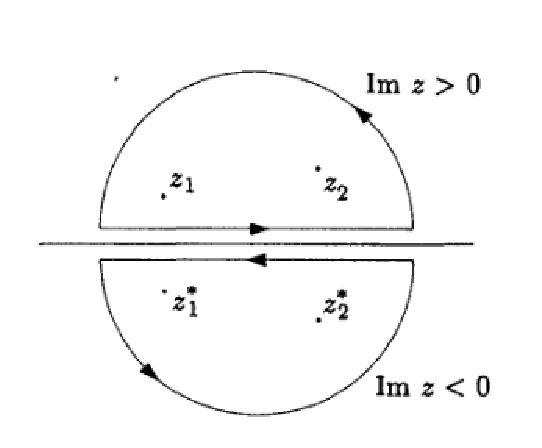
\includegraphics[height=50mm]{contours}  
  \caption{Объединение контуров интегрирования в тождесте Уорда в граничной конформной теории поля}
  \label{fig:ward}
\end{figure}

То есть если нас интересует $n$-точечная корреляционная функция в теории на верхней полуплоскости, мы можем рассматривать голоморфную часть $2n$-точечной функции на всей плоскости. Взаимодействие полей с границей симулируется путем рассмотрения взаимодействия полей с их зеркальными отражениями. 

Если мы хотим изучать теорию с неоднородными граничными условиями, мы можем сделать это введя так называемые граничные операторы. Рассмотрим, для примера, поле $\phi(z)$  с конформной размерностью $h$, заданное на верхней полуплоскости. При приближении к вещественной оси оно взаимодействует со своим зеркальным отражением и мы можем воспользоваться операторным разложением:
\begin{equation}
  \label{eq:176}
  \phi(z)\phi(z^*)\approx \sum_i (z-z^*)^{(h_i -2h)}\varphi_B^{(i)}(x),
\end{equation}
где мы отбросили высшие члены и положили $x=\frac{z+z^*}{2}$, а поля $\varphi_B$ живут на границе. Операторы $\varphi_B^{(i)}$ можно рассматривать как операторы изменения граничных условий.  Их классификация следует из требований модулярной инвариантности и дается формулой Верлинде (См. \cite{cardy1989boundary,difrancesco1997cft}). 

Аналогичные рассуждения можно провести для ВЗНВ- и coset-моделей на верхней полуплоскости \cite{gawedzki2002boundary},\cite{ishikawa2003novel}, \cite{fuchs2005geometry,fredenhagen2002d,elitzur2002d,felder1999geometry,alekseev1999d}, \cite{mercat2001integrable}.

В разделе \ref{sec:SLE} мы обсудим связь граничной конформной теории поля с решеточными моделями и стохастическими процессами. 

\section{Аффинные алгебры Ли в моделях Весса-Зумино-Новикова-Виттена }
\label{sec:WZNW-models}

Модели Весса-Зумино-Новикова-Виттена обладают дополнительной симметрией. Алгебра токов в них --- это алгебра Каца-Муди
(аффинная алгебра Ли $\mathfrak{g}$), полная киральная алгебра --- полупрямое произведение
$Vir\ltimes \mathfrak{g}$, примарные поля классифицируются по неприводимым представлениям алгебры $\mathfrak{g}$.

В данном разделе мы показываем, как такие модели можно строить путем квантования нелинейной сигма-модели с дополнительным членом Весса-Зумино следуя обзору \cite{Walton:1999xc} и книге \cite{difrancesco1997cft}. 

Модели Весса-Зумино-Новикова-Виттена можно строить начиная со следующего действия:
\begin{equation}
\label{eq:4}
  S=S_0+k\Gamma
\end{equation}
где $k$ - целое.
Здесь $S_0$ --- действие нелинейной $\sigma$-модели.
\begin{equation}
  \label{eq:5}
  S_0=\frac{1}{4a^2}\int_{S^2} d^2x\; Tr (\partial^{\mu}g^{-1}\partial_{\mu}g),
\end{equation}
где $a^2>0$ - положительный параметр, $g(x)\in G$ - поле со значениями в группе Ли $G$, которую мы
будем считать полупростой. Действие задается на комплексной плоскости с бесконечностью, которая
топологически эквивалентна 2-сфере. Взятие следа $Tr$ представляет собой матричную реализацию формы Киллинга ${\cal K}$ алгебры Ли $\gf$, соответствующей группе Ли $G$.

В нелинейной $\sigma$-модели конформная инвариантность теряется на квантовом уровне.
Голоморфный и антиголоморфный токи не сохраняются по отдельности.
Поэтому мы добавляем член Весса-Зумино $\Gamma$ к действию
\begin{equation}
  \label{eq:73}
\Gamma= - \frac{i }{24\pi} \int_{B}\epsilon_{ijk} Tr\left(
    \tilde g^{-1}\frac{\partial \tilde g}{\partial y^i}
      \tilde g^{-1}\frac{\partial \tilde g}{\partial y^j}
      \tilde g^{-1}\frac{\partial \tilde g}{\partial y^k}\right) d^3y
\end{equation}
Он определен на трехмерном многообразии $B$, ограниченном исходным двумерным пространством $S^{2}$.
Через $\tilde{g}$ мы обозначили продолжение поля $g$ на $B$. Такое продолжение не единственно. В
компактифицированном трехмерном пространстве компактное двумерное многообразие разделяет два
трехмерных многообразия.
\begin{figure}[h]
 \centering
  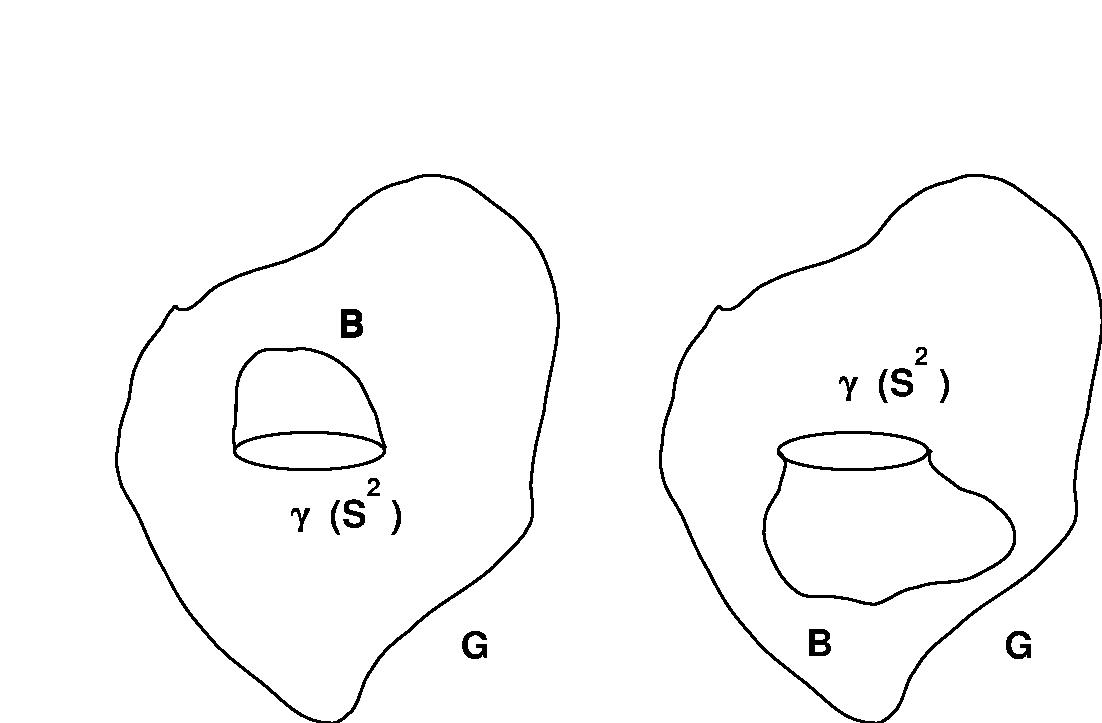
\includegraphics[width=100mm]{fig3}  
  \caption{Два продолжения поля на трехмерное многообразие}
  \label{fig:1}
\end{figure}

Разность значений члена Весса-Зумино $\Delta\Gamma$ на этих многообразиях
дается правой частью уравнения (\ref{eq:73}) с интегралом, продолженным на все компактное трехмерное
пространство. Так как оно топологически эквивалентно три-сфере, получаем
\begin{equation}
  \label{eq:75} \Delta\Gamma= - \frac{i }{24\pi} \int_{S^3}\epsilon_{ijk} Tr\left( \tilde
g^{-1}\frac{\partial \tilde g}{\partial y^i} \tilde g^{-1}\frac{\partial \tilde g}{\partial y^j}
\tilde g^{-1}\frac{\partial \tilde g}{\partial y^k}\right) d^3y
\end{equation}
$\Delta\Gamma$ определен по модулю $2\pi i$, поэтому Евклидов функциональный интеграл
с весом $exp(-\Gamma)$ хорошо определен. Значит константа связи, умножаемая на этот член, должна
быть целочисленной.

Уравнение движения для полного действия (\ref{eq:4}):
\begin{equation}
  \label{eq:77}
  \partial^{\mu}(g^{-1}\partial_{\mu}g)+\frac{a^2 ik}{4\pi}\epsilon_{\mu\nu}\partial^{\mu}(g^{-1}\partial^{\nu}g)=0
\end{equation}
В комплексных координатах оно записывается в виде
\begin{equation}
  \label{eq:78}
  \left(1+\frac{a^2 k}{4\pi}\right)\partial_z(g^{-1}\partial_{\bar z}g)+\left(1-\frac{a^2 k}{4\pi}\right)\partial_{\bar z}(g^{-1}\partial_z g)=0
\end{equation}
Видно, что при $a^2=\frac{4\pi}{k}$ у нас имеются законы сохранения
\begin{equation}
  \label{eq:79}
  \partial_z(g^{-1}\partial{\bar z}g)=0
\end{equation}
Введем токи
\begin{equation}
  \label{eq:72}
  J_z=\partial_z g\;g^{-1}, \qquad J_{\bar{z}}=g^{-1}\partial{\bar z}g.
\end{equation}
Тогда уравнение (\ref{eq:79}) примет вид
\begin{equation}
  \label{eq:100}
  \partial_{\bar z}J=0,\quad \partial_z \bar J=0
\end{equation}
То есть голоморфная и антиголоморфная части отщепляются, что является указанием на наличие
конформной инвариантности.

Решение классического уравнения движения имеет вид
\begin{equation}
  \label{eq:80}
  g(z,\bar z)=f(z)\bar f(\bar z)
\end{equation}
при произвольных $f(z)$ и $\bar f (\bar z)$.

Сохранение по отдельности токов $J_z,\; J_{\bar z}$ приводит к инвариантности действия при преобразованиях
\begin{equation}
  \label{eq:81}
   g(z,\bar z)\to \Omega(z)g(z,\bar z)\bar \Omega^{-1}(\bar z)
\end{equation}
где $\Omega,\;\bar \Omega \in G$. То есть мы получили локальную $G(z)\times G(\bar z)$-инвариантность.

Для перехода к квантовому случаю мы переопределяем токи
\begin{equation}
  \label{eq:82}
  J(z)\equiv -k \partial_zg g^{-1}\quad \bar J(\bar z)=k g^{-1}\partial_{\bar z}g
\end{equation}
 При инфинитезимальных преобразованиях $\Omega=1+\omega,\; \bar \Omega =1+\bar \omega$ вариация поля
 $\delta_{\omega}g=\omega g$, а вариация действия дается равенством
 \begin{equation}
   \label{eq:11}
   \delta S=-\frac{1}{2\pi}\int d^2 x \left(\partial_{\bar z}Tr(\omega(z)J(z))+\partial_z Tr(\bar
     \omega(\bar z)\bar J(\bar z))\right)
 \end{equation}
Заменяем $d^2 x=-\frac{i}{2} dz d\bar z$, интегрируем по частям и переходим к интегралу по контуру, замыкая
контур в разных направлениях для голоморфной и антиголоморфной частей.
Тогда вариация действия примет вид
\begin{equation}
  \label{eq:83}
  \delta_{\omega,\bar\omega}S=\frac{i}{4\pi}\oint dz Tr (\omega(z)J(z))-\frac{i}{4\pi}\oint d\bar z Tr(\bar\omega(\bar z)\bar J(\bar z))
\end{equation}
Раскладывая токи по некоторому базису $t^{a}$ в алгебре Ли $\gf$
\begin{equation}
  \label{eq:85}
  \begin{aligned}
    J=\sum J^a t^a,\bar J=\sum \bar J^a t^a \\
    \omega=\sum \omega^a t^a\\
  \end{aligned}
\end{equation}
получаем
\begin{equation}
  \label{eq:86}
  \delta_{\omega,\bar \omega}S=-\frac{1}{2\pi i}\oint dz \sum\omega^a J^a+\frac{1}{2\pi i} \oint d\bar z \sum \bar \omega^a \bar J^a
\end{equation}
Мы также получили тождества Уорда $\delta\left< X\right>=\left<(\delta S)X\right>$
\begin{equation}
  \label{eq:87}
  \delta_{\omega,\bar \omega}\left< X \right>=-\frac{1}{2\pi i}\oint dz \sum\omega^a \left< J^a X\right>+
  \frac{1}{2\pi i} \oint d\bar z \sum \bar \omega^a \left< \bar J^a X\right>
\end{equation}
Из явного вида тока и формулы для преобразования $g$ имеем
\begin{equation}
  \label{eq:88}
  \delta_{\omega}J=[\omega,J]-k\partial_z\omega,\quad \delta_{\omega}J^a=\sum i f_{abc}\omega^b J^c-k\partial_z\omega^a
\end{equation}
Если это подставить в тождество Уорда, то получаем операторное разложение для токов:
\begin{equation}
  \label{eq:89}
  J^a(z) J^b(w) \sim \frac{k\delta_{ab}}{(z-w)^2}+\sum i f_{abc}\frac{J^c(w)}{(z-w)}
\end{equation}
Раскладывая токи в ряд, получаем
\begin{equation}
  \label{eq:90}
  \begin{aligned}
    J^a(z)=\sum_{n\in \mathbb Z}z^{n-1}J^a_n\\
    \left[J^a_n,J^b_m\right]=\sum_c i f^{abc}J^c_{n+m}+kn\delta^{ab}\delta_{n+m,0}
  \end{aligned}
\end{equation}
Теперь мы видим, что компоненты токов образуют аффинную алгебру Ли $\hat g$.


Тензор энергии-импульса вводится при помощи конструкции Сугавары как сумма нормально упорядоченных компонент токов
\begin{equation}
  \label{eq:102}
  T(z)=\frac{1}{2(k+h^{\vee})}\sum_a :J^a J^a:(z)
\end{equation}
Здесь $h^{\vee}$ - дуальное число Кокстера. $h^{\vee}=\sum_i \alpha_i^{\vee} +1=\frac{1}{2}(\theta,\theta+2\rho)$,
а нормальное упорядочение вводится следующим образом: 
\begin{equation}
  \label{eq:12}
  :AB:(w)=\frac{1}{2\pi i}\oint\frac{dz}{z-w}A(z)B(w)
\end{equation}

Тензор энергии-импульса можно разложить на моды $L_n$
\begin{equation}
  \label{eq:91}
  L_n=\frac{1}{2(k+h^{\vee})}\sum_a\sum_m:J^a_m J^a_{n-m}:
\end{equation}
Тогда коммутационные соотношения для мод $L_n$ имеют вид
\begin{equation}
  \label{eq:92}
  \begin{aligned}
    \left[L_n,L_m\right]=(n-m)L_{n+m}+\frac{c}{12}(n^3-n)\delta_{n+m,0}\\
    c=\frac{k\;\mathrm{dim}g}{k+h^{\vee}}\\
    \left[L_n,J^a_m\right]=-mJ^a_{n+m}.
  \end{aligned}
\end{equation}

Таким образом, конструкция Сугавары --- это способ вложения алгебры Вирасоро в универсальную обертывающую аффинной алгебры Ли $\hat{g}$

Полная киральная алгебра модели Весса-Зумино-Виттена равна полупрямому произведению $Vir\ltimes \hat g$

Примарными назваются поля, которые преобразуются ковариантно под действием $G(z)\times G(\bar z)$,
как $g(z,\bar z)$. В терминах операторного разложения это свойство переформулируется следующим
образом:
\begin{equation}
  \label{eq:84}
  \begin{aligned}
    J^a(z)g(w,\bar w)\sim \frac{-t^a g(w,\bar w)}{(z-w)}\\
    \bar J^a(z)g(w,\bar w)\sim \frac{ g(w,\bar w)t^a}{(z-w)}
  \end{aligned}
\end{equation}
Любое поле $\phi_{\lambda,\mu}$, преобразующееся ковариантно по отношению к некоторому
представлению, заданному весом $\lambda$ в голоморфном секторе и весом $\mu$ в антиголоморфном,
является примарным полем WZW-модели.

В модах это свойство записывается в виде
\begin{equation}
  \label{eq:93}
  \begin{aligned}
    & (J_0^a \phi_{\lambda})=-t^a_{\lambda}\phi_{\lambda}\\
    & (J^a_n\phi_{\lambda})=0\quad \mbox{для}\; n>0\\
  \end{aligned}
\end{equation}
Мы можем сопоставить состояние $\left|\phi_{\lambda}\right>$ полю $\phi_{\lambda}$
  \begin{equation}
    \label{eq:94}
    \left|\phi_{\lambda}\right>=\lim_{z\to 0}\phi_{\lambda}(z)\left|0\right>
  \end{equation}
Тогда условия (\ref{eq:93}) для примарных полей дают
\begin{equation}
  \label{eq:95}
  \begin{aligned}
    & J_0^a\left|\phi_{\lambda}\right>=-t^a_{\lambda}\left|\phi_{\lambda}\right>\\
    & J^a_n\left|\phi_{\lambda}\right>=0 \quad \mbox{для}\; n>0 \\
  \end{aligned}
\end{equation}
Все вторичные состояния имеют вид
\begin{equation}
  \label{eq:97}
  J^{a_1}_{-n_1}J^{a_2}_{n_2}\dots\left|\phi_{\lambda}\right>
\end{equation}

Легко видеть, что действие генераторов алгебры Вирасоро на примарные поля имеет вид
\begin{equation}
  \label{eq:96}
  L_0\left|\phi_{\lambda}\right>=\frac{1}{2(k+h^{\vee})}\sum_aJ^a_0J^a_0\left|\phi_{\lambda}\right>=\frac{(\lambda,\lambda+2\rho)}{2(k+h^{\vee})}\left|\phi_{\lambda}\right>
\end{equation}
Здесь использовано явное выражение для собственных значений квадратичного оператора Казимира. То есть конформный вес примарного поля ВЗНВ-модели равен
\begin{equation}
  \label{eq:65}
  h_{\lambda}=\frac{(\lambda,\lambda+2\rho)}{2(k+h^{\vee})}
\end{equation}


%Примарные поля преобразуются  интегрируемыми конечномерными представлениями, а бесконечномерные и
%неинтегрируемые поля зануляют корреляционные функции.
В WZW-моделях примарные поля
принадлежат тензорному произведению неприводимых представлений аффинной алгебры, так как есть
голоморфный и антиголоморфный сектора.

Из тождества Уорда для токов \eqref{eq:87}, конструкции Сугавары \eqref{eq:102} и операторного разложения для тока и примарного поля \eqref{eq:84} нетрудно получить уравнение Книжника-Замолодчикова на корреляционные функции:
\begin{equation}
  \label{eq:66}
  \left( \frac{\partial}{\partial z_i}+\sum_{j\neq i}^N \sum_a \frac{t^a_i t^a_j}{k+h^{\vee}}\frac{1}{z_i-z_j}\right) \langle g (z_1,\bar z_1)\dots g(z_N,\bar z_N)\rangle
\end{equation}
Решая эти уравнения, в принципе, можно найти все корреляционные функции. 

Как мы видим, теория представлений аффинных алгебр Ли играет определяющую роль при изучении моделей Весса-Зумино-Новикова-Виттена. Для удобства приведем в следующем разделе основные определения.

\subsection{Простые алгебры Ли, алгебра петель, центральные расширения и аффинные алгебры Ли}

\label{sec:intro-simple-lie-algebras}
\begin{definition}
{\it Алгебра Ли $\gf$} -- это векторное пространство с билинейной операцией $[\cdot,\cdot]:\gf\otimes\gf\to \gf$, которая называется  {\it скобкой Ли или коммутатором}. Если выбрать некоторый базис  $X_{i}$ в $\gf$, то коммутационные соотношения можно задать при помощи  {\it структурных констант} $C_{ijk}$:
\begin{equation}
  \label{eq:1}
  [X^{i},X^{j}]=\sum_{k} C^{ij}_{k} X^{k}
\end{equation}
  
\end{definition}

Алгебра Ли называется {\it простой} если она не содержит нетривиальных идеалов относительно коммутатора. {\it Полупростая} алгебра Ли -- это прямая сумма простых алгебр Ли. 

{\it Подалгеброй Картана}  $\hfg$ называется нильпотентная подалгебра алгебры $\gf$, совпадающая со своим нормализатором. Мы обозначаем элементы базиса в $\hfg$ через $H^{i}$.

Форма Киллинга ${\cal K}$ на  $\gf$ порождает невырожденную билинейную форму $(\cdot,\cdot)$ на подалгебре Картана $\hfg$, позволяющую идентифицировать $\hfg$ с подпространством дуального пространства  $\hfg^{*}$ линейных функционалов на $\hfg$. {\it Веса}  -- это элементы  $\hfg^{*}$, мы обозначаем их греческими буквами $\mu,\nu, \omega, \lambda\dots$


Коммутационные соотношения  (\ref{eq:1}) можно записать в компактной форме, если выбрать базис специальным образом. Такой базис описывается корневой системой, которая определяется в разделе \ref{sec:weights-roots} (Смотри также \cite{humphreys1997introduction,humphreys1992reflection}).

Чтобы определить аффинные алгебры нам нужно обсудить процедуру центрального расширения алгебры Ли.
Напомним несколько определений (см \cite{fuks1986cohomology},\cite{fuks1984}, \cite{feigin1988}).
\begin{definition}
\label{def:1}
Будем рассматривать алгебру Ли $\gf$ над полем $k=\mathbb{C},\mathbb{R}$. Векторное пространство $A$ над полем $k$ называется {\it модулем над $\gf$} или {\it $\gf$-модулем}, если задано билинейное отображение $\mu:\gf\times A\to A$, такое что $\mu([X,Y],a)=\mu(X,\mu(Y,a))-\mu(Y,\mu(X,a))$ для $X,Y\in \gf, a\in A$. Далее мы будем опускать символ $\mu$ и писать $X a= \mu(X,a)$.
\end{definition}
\begin{definition}
  {\it $n$-мерная коцепь с коэффициентами в $A$} -- это кососимметричный $n$-линейный функционал на $\gf$ со значениями в $A$. Пространство $n$-коцепей $C^{n}(\gf;A)=\mathrm{Hom}(\wedge^{n}\gf;A)$.
\end{definition}
Заметим, что элементы $\gf$ действуют на $C^{n}(\gf;A)$.
\begin{definition}
  Внешний дифференциал $d=d_{n}:C^{n}(\gf;A)\to C^{n+1}(\gf;A)$ определяется формулой
  \begin{multline}
    \label{eq:68}
    (dc) (X_{1},\dots, X_{n+1})=\sum_{1\leq s<t\leq n+1} (-1)^{s+t-1} c([X_{s},X_{t}],X_{1},\dots,\hat X_{s},\dots,\hat X_{t},\dots X_{n+1})\\
    +\sum_{1\leq s\leq n+1} (-1)^{s}X_{s} c(X_{1},\dots \hat X_{s},\dots X_{n+1})
  \end{multline}
\end{definition}
Нетрудно проверить, что последовательность
\begin{equation}
  \label{eq:40}
  \dots\stackrel{d_{n}}{\longleftarrow} C^{n}(g;A)\stackrel{d_{n-1}}{\longleftarrow} C^{n-1}(\gf;A)\leftarrow \dots \leftarrow C^{1}(\gf;A) \stackrel{d_{0}}{\longleftarrow} C^{0}(\gf;A)\leftarrow 0
\end{equation}
точна.Тогда $\{C^{n}(\gf;A),d_{n}\}=C^{*}(\gf;A)$ есть комплекс.
\begin{definition}
Соответствующие когомологии называются {\it когомологиями алгебры $\gf$ с коэффициентами в $A$} и обозначаются через $H^{n}(\gf;A)=\mathrm{Ker}\; d_{n}/\mathrm{Im}\; d_{n-1}$. 
  
\end{definition}
Заметим, что поле $k$ может рассматриваться как тривиальный $\gf$-модуль. В этом случае второй член в формуле \eqref{eq:1} исчезает и используют сокращенные обозначения $C^{n}(\gf), H^{n}(\gf)$.
\begin{definition}
  Определим, заодно, и гомологии. Пространство $n$-мерных цепей $C_{n}(\gf;A)=A\otimes \wedge^{n}\gf$, дифференциал $\partial=\partial_{n}:C_{n}(\gf;A)\to C_{n-1}(\gf;A)$ определяется формулой
  \begin{multline}
    \label{eq:98}
    \partial(a\otimes (X_{1}\wedge \dots \wedge X_{n})) =\\ \sum_{1\leq s<t\leq n+1} (-1)^{s+t-1} a\otimes ([X_{s},X_{t}]\wedge X_{1} \wedge\dots\wedge\hat X_{s}\wedge \dots\wedge \hat X_{t}\wedge \dots\wedge X_{n+1})\\
    +\sum_{1\leq s\leq n+1} (-1)^{s}(X_{s} a)\otimes (X_{1}\wedge\dots\wedge \hat X_{s}\wedge\dots\wedge X_{n+1})
  \end{multline}
  Аналогично определяется точная последовательность, комплекс и группа гомологий $H_{n}(\gf;A)$.
\end{definition}
\begin{definition}
  {\it Одномерным центральным расширением алгебры $\gf$ } называется точная последовательность
  \begin{equation}
    \label{eq:62}
    0\to k \to \tilde \gf\to \gf\to 0,
  \end{equation}
  такая что образ $k\to \tilde\gf$ содержится в центре $\tilde\gf$.
\end{definition}
Заметим, что всякий 2-коцикл $c\in C^{2}(\gf;A), \; dc=0$ определяет центральное расширение $\gf$:
\begin{equation}
  \label{eq:64}
  0\to k\stackrel{\lambda\to (0,\lambda)}{\longrightarrow}\tilde\gf=\gf\oplus k \stackrel{(X,\lambda)\to X}{\longrightarrow} \gf\to 0
\end{equation}
Скобка Ли в алгебре $\tilde\gf$, которая равна $\gf\oplus k$ как векторное пространство, определяется равенством
\begin{equation}
  \label{eq:103}
  [(X,\lambda),(Y,\mu)]=([X,Y],c(X,Y))
\end{equation}
Тождество Якоби для такой скобки равносильно тому, что $c$\; --- 2-коцикл. Когомологичным коциклам отвечают эквивалентные расширения. 

Два расширения $\tilde \gf$ и $\tilde{\tilde\gf}$ называются эквивалентными, если существует изоморфизм $I:\tilde\gf\to \tilde{\tilde \gf}$ такой, что диаграмма коммутирует:
\begin{equation}
  \label{eq:104}
  \begin{diagram}
    \node 0 \arrow{e,t}{}  \node{\gf} \arrow{e,t}{} \arrow{s,l}{id} \node{\tilde\gf}\arrow{s,l}{I} \arrow{e,t}{} \node{k}\arrow{s,r}{id} \arrow{e,t}{} \node{0}\\
    \node 0 \arrow{e,t}{}  \node{\gf} \arrow{e,t}{} \node{\tilde{\tilde\gf}} \arrow{e,t}{} \node{k} \arrow{e,t}{} \node{0}
  \end{diagram}
\end{equation}
%% \begin{exercise}
%%  Построить изоморфизм $I$.   
%% \end{exercise}


Таким образом пространство $H^{2}(\gf)$ -- это множество классов 1-мерных центральных расширений $\gf$. Нуль в $H^{2}(\gf)$  соответствует тривиальному расширению. 

Для алгебры Витта \eqref{eq:2} существует коцикл
\begin{equation}
  \label{eq:105}
  c(l_{n},l_{m})=\frac{1}{12}(m^{3}-m)\delta_{-n,m}
\end{equation}
%% \begin{exercise}
%%   Проверить, что $c$ -- коцикл алгебры Витта. 
%% \end{exercise}
Соответствующее центральное расширение алгебры Витта называется алгеброй Вирасоро. Коммутационные соотношения этой алгебры имеют вид
\begin{eqnarray}
  \label{eq:106}
  [L_{n},c]=0\\
  \left[L_{n},L_{m}\right]=(n-m)L_{n+m} +\frac{c}{12} (m^{3}-m) \delta_{-n,m}
\end{eqnarray}
Можно показать, что $H^{2}(Witt)\cong \mathbb{C}$ и все нетривиальные коциклы пропорциональны $c$. 
(Доказательство есть в \cite{fuks1986cohomology}, \cite{schottenloher2008mathematical}).

{\it Алгебра петель} $L\gf=\gf\otimes \mathbb{C}[t,t^{-1}]$, соответствующая полупростой алгебре Ли $\gf$, определяется коммутационными соотношениями
\begin{equation}
  \label{eq:108}
  [X^{i}t^{n},X^{j}t^{m}]=t^{n+m}\sum_{k}C^{ij}_{k}X^{k}
\end{equation}
Центральное расширение алгебры петель ведет к возникновению дополнительного члена
\begin{equation}
  \label{eq:112}
   [X^{i}t^{n}+\alpha c,X^{j}t^{m}+\beta c]=t^{n+m}\sum_{k}C^{ij}_{k}X^{k}+(X^{i},X^{j})n\delta_{n+m,0}c
\end{equation}
Эта алгебра $\hat\gf=\gf\otimes\mathbb{C}[t,t^{-1}]\oplus\mathbb{C}c$ называется (не скрученной)  {\it аффинной алгеброй Ли} \cite{kac1990idl}, \cite{wakimoto2001idl,wakimoto2001lectures}, \cite{kass1990ala}.

\subsubsection{Модули, веса и корни}
\label{sec:weights-roots}

Пусть $\gf$ -- конечномерная или аффинная алгебра Ли. Мы ввели модули алгебры $\gf$ в определении \ref{def:1}. Широко используется альтернативный термин {\it представление}.

%%    $\gf$-модулем называется векторное пространство $V$ с билинейным отображением $\gf \times V\to V$, таким, что выполнено равенство
%%  \begin{equation}
%%    \label{eq:130}
%%    [x,y]\cdot v = x\cdot(y\cdot v) - y\cdot(x\cdot v), \quad \mbox{for}\; x,y\in \gf, v\in V
%%  \end{equation}
\begin{definition}
Представление алгебры  $\gf$ на векторном пространстве $V$ называется гомоморфизм $\gf\to gl(V)$ из $\gf$ в алгебру Ли эндоморфизмов векторного пространства $V$, где скобка задана коммутатором:
\begin{equation}
  \label{eq:113}
  [x,y]\cdot v = x\cdot(y\cdot v) - y\cdot(x\cdot v), \quad \mbox{для}\; x,y\in \gf, v\in V  
\end{equation}

\end{definition}

В произвольном представлении операторы, соответствующие генераторам подалгебры Картана $H^{i}$, можно одновременно диагонализовать путем специального выбора базиса
 $\{v_{j}\}$ в $V$:
\begin{equation}
  \label{eq:114}
  H^{i}\cdot v_{j}=\nu_{j}^{i}v_{j}
\end{equation}
Собственные значения $\nu^{i}_{j}$ генераторов Картана на элементе базиса $v_{j}$ определяют вес  $\nu_{j}\in \hfg^{*}$, такой, что $\nu_{j}(H^{i})=\nu_{j}^{i}$. Вектор $v\in V$ называется весовым вектором веса  $\lambda$, если $H v=\lambda_{j}(H)v,\; \forall H\in \hf$. Весовое подпространство состоит из всех весовых векторов $V_{\lambda}=\{v\in V: H v=\lambda_{j}(H)v,\; \forall H\in \hf\}$. Кратностью веса  $m_{\lambda}=\mathrm{mult}(\lambda)=\mathrm{dim} V_{\lambda}$ называется размерность весового подпространства.

Структура модуля определяется набором весов, так как действие генераторов $E^{\alpha}$ на весовых векторах дается выражением
\begin{equation}
  \label{eq:115}
  E^{\alpha}\cdot v_{\lambda} \propto v_{\lambda+\alpha}
\end{equation}

Структуру модуля можно записать в виде формального характера
\begin{equation}
  \label{eq:116}
  \mathrm{ch}V=\sum_{\lambda}m_{\lambda} e^{\lambda}
\end{equation}
Характер  $\mathrm{ch}V\in \mathcal{E}$ -- это элемент алгебры  $\mathcal{E}$, порожденной формальными экспонентами весов. Характер можно специализировать --- взять его значение на некотором элементе $\xi\in\hf$.

Алгебра Ли является собственным модулем по отношению к специальному представлению, называющемуся присоединенном. Действие генераторов в этом представлении дается скобкой $ad_{X} Y=[X,Y]$. 
{\it Корни} -- это веса присоединенного представления алгебры $\gf$.  Они определяют коммутационные соотношения в алгебре следующим образом. Обозначим через $\Delta$ множество корней. Для каждого $\alpha\in \Delta$ существует корень  $-\alpha\in \Delta$ и генераторы $E^{\alpha}, E^{-\alpha}$, такие, что
\begin{align}
  \label{eq:63}
  &  [H^{i},E^{\alpha}]=\alpha^{i}E^{\alpha} \\
  &\left[E^{\alpha},E^{\beta}\right]=
  \begin{cases}
    N_{\alpha,\beta} E^{\alpha+\beta}, & \mbox{if}\; \alpha+\beta\in \Delta\\
    \frac{2}{(\alpha,\alpha)} \sum_{i}\alpha^{i} H^{i},&  \mbox{if}\; \alpha=-\beta\\
    0,&\mbox{в остальных случаях}
  \end{cases}
\end{align}

В корневой системе $\Delta$ можно выбрать множество {\it положительных корней}. Это подмножество  $\Delta^{+}\subset \Delta$, такое, что для любого корня $\alpha\in\Delta$ ровно один из корней $\alpha, -\alpha$ содержится $\Delta^{+}$ и для любых двух различных положительных корней $\alpha, \beta\in \Delta^{+}$, таких, что $\alpha+\beta\in \Delta$ их сумма тоже положительна $\alpha+\beta\in\Delta^{+}$.
Элементы множества $-\Delta^{+}$ называются отрицательными корнями.

\begin{definition}
\label{def:singular-weight}
  {\it Сингулярным} называется вектор $v_{\lambda}$, такой что $E^{\alpha}v_{\lambda}=0,\; \forall \alpha\in \Delta^+$. Вес $\lambda$, отвечающий сингулярному вектору, также называется сингулярным. 
\end{definition}
В следующем разделе мы показываем, что структура модулей старшего веса определяется сингулярным элементом -- элементом алгебры, порожденной формальными экспонентами весов, который является линейной комбинацией экспонент сингулярных весов. 

Положительный корень называется {\it простым} если его нельзя представить в виде суммы положительных корней. Множество простых корней  $\Phi=\left\{\alpha_{i}\right\}$ является базисом в $\hfg^{*}$ и каждый корень может быть записан как сумма $\alpha=\sum_{i}n_{i}\alpha_{i}$, где все $n_{i}$ не отрицательны или не положительны одновременно. В случае конечномерной алгебры Ли  $\gf$ простые корни можно пронумеровать числами от  1 до ранга алгебры $i=1,\dots,r,\quad r=\mathrm{rank}(\gf)$. Такая нумерация порождает лексикографическое упорядочение корневой системы. Старший по отношению к этому упорядочению корень обозначается через $\theta=\sum_{i=1,\dots,r} a_i \alpha_i$, его координаты в базисе простых корней $a_i$ называются  {\it марками}. $\theta$ -- это старший вес присоединенного модуля (См. раздел \ref{sec:high-weight-modul}). {\it Ко-марками} называются числа $a_i^{\vee}=\frac{(\alpha_i,\alpha_i)}{2} a_i$.

В аффинной алгебре Ли  $\hat\gf$ множество корней  $\Delta$ бесконечно, но набор простых корней  $\Phi$ конечен. Обозначим его элементы через $\alpha_{0},\dots \alpha_{r}$, где $r=\mathrm{rank}(\gf)$. Корни $\alpha_1,\dots, \alpha_r$ -- это корни соответствующей конечномерной алгебры Ли $\go$. Простой корень  $\alpha_0=\delta-\theta$ -- это разность  {\it мнимого корня} $\delta$ и $\theta$ -- старшего корня алгебры $\go$.
Заметим, что кратность корня  $\mathrm{mult}(\alpha)$ в случае аффинной алгебры Ли может быть больше единицы.

Подалгебра  $\bff_{+}\subset \gf$, порожденная генераторами $H^{i}, E^{\alpha}$, соответствующими положительным корням $\alpha\in \Delta^{+}$, называется подалгеброй Бореля.

{\it Параболическая подалгебра}  $\pf_{I}\supset \bff_{+}$ содержит подалгебру Бореля и порождена некоторым подмножеством простых корней  $\{\alpha_{j}:j\in I, I\subset \{1\dots r\}\}$. Она образована подмножеством генераторов  $\{H^{i}\}\cup \{E^{\alpha}:\alpha\in \Delta^{+}\}\cup \{E^{-\alpha}: \alpha\in\Delta^{+}, \alpha=\sum_{j\in I} n_{j} \alpha_{j}\}$.
{\it Регулярная подалгебра} $\af\subset\gf$ определяется корневой системой  $\Delta_{\af}$, множество простых корней которой  $\{\beta_{i}, i=1,\dots,r_{\af}\}$ является подмножеством множества $\{\alpha_{1},\dots,\alpha_{r}\}\cup \{-\theta\}$ корней алгебры $\gf$.

 {\it Группа Вейля} $W_{\gf}$ порождается отражениями $\{s_{i}:\hfg^{*}\to\hfg^{*}\}$, соответствующим простым корням $\{\alpha_{i}\}$:
\begin{equation}
  \label{eq:117}
  s_{i}\cdot\lambda=\lambda-\frac{2(\alpha_{i},\lambda)}{(\alpha_{i},\alpha_{i})}\alpha_{i}
\end{equation}
Корневая система и характеры представлений инвариантны относительно действия группы Вейля. Корневая система может быть восстановлена из множества простых корней в результате применения вейлевских отражений.

Группа Вейля конечна для конечномерных алгебр Ли и конечно порождена для аффинных алгебр Ли.

Рассмотрим действие элемента группы Вейля $s_{\alpha}s_{\alpha+\delta}$ аффинной алгебры Ли   $\hat\gf$, соответствующего простому корню  $\alpha$ конечномерной подалгебры Ли $\gf$. Из определения  \eqref{eq:117} легко видеть, что $s_{\alpha}s_{\alpha+\delta} \cdot \lambda=\lambda+\frac{2}{(\alpha,\alpha)}\alpha+\left(\frac{(\alpha,\alpha)}{2 (\lambda,\delta)}+(\lambda,\alpha)\right) \delta$. То есть группа Вейля для аффинной алгебры Ли может быть представлена как полупрямое произведение группы Вейля $W_{\gf}$ конечномерной подалгебры  $\gf$ и трансляций, соответствующих корням $\gf$. 

Элемент группы Вейля можно представить как произведение простых отражений различными способами. Число простых отражений в кратчайшей последовательности, представляющей элемент\; $w\in W_{\gf}$ называется {\it длиной}  $w$ и обозначается $l(w)$. Мы также используем обозначение $\epsilon(w)=(-1)^{l(w)}$ для четности числа отражений Вейля, порождающих $w$. 

Фундаментальная область $\bar{C}$ для действия группы Вейля $W_{\gf}$ на $\hfg^{*}$ описывается условием $\xi\in \bar{C}\Leftrightarrow (\xi,\alpha_{i})\geq 0$ для всех простых корней $\alpha_{i}$. Ее называют {\it главной камерой Вейля}. 

{\it Матрица Картана} $A$ строится из произведений простых корней
\begin{equation}
  \label{eq:118}
  A_{ij}=\frac{2(\alpha_{i},\alpha_{j})}{(\alpha_{j},\alpha_{j})}.
\end{equation}
Она может использоваться для компактного описания алгебры Ли и ее коммутационных соотношений в базисе Шевалле \cite{humphreys1997introduction}, \cite{fulton1991representation}, \cite{bourbaki2002lie}.

Форма, заданная матрицей Картана \eqref{eq:118} определяет базис, дуальный к базису простых корней.  Он называется  {\it базисом фундаментальных весов}. Мы обозначаем его элементы через $\omega_i$:
\begin{equation}
  \label{eq:20}
  \langle\omega_i,\alpha_j\rangle=\frac{2(\omega_{i},\alpha_{j})}{(\alpha_{j},\alpha_{j})}=\delta_{ij}
\end{equation}
Для конечномерной алгебры Ли существует $r$ фундаментальных весов $\omega_{i}$, $i=1,\dots, r$. Для аффинной алгебры Ли есть дополнительный фундаментальный вес $\omega_0=\lambda$, $(\lambda,\delta)=1, \; (\lambda,\lambda)=(\delta,\delta)=0$. Другие фундаментальные веса равны $\omega_i=a_i^{\vee} \omega_0 +\co{\omega_i}$, где $\co{\omega_i}$ -- это фундаментальные веса конечномерной подалгебры Ли $\gf$.

Сумма фундаментальных весов $\rho=\sum_{i} \omega_{i}$ называется {\it вектором Вейля} и играет большую роль в теории представлений.

\subsubsection{Модули старшего веса}
\label{sec:high-weight-modul}

Мы рассматриваем конечно-порожденные  $\gf$-модули $V$, такие, что $V=\bigoplus_{\xi\in \hfg^{*}} V_{\xi}$, где каждое подпространство $V_{\xi}$ конечномерно и существует конечный набор весов $\lambda_{1},\dots \lambda_{s}$, порождающий весовую систему модуля $V$. То есть, если $\mathrm{dim}V_{\xi}\neq 0$, то $\xi=\lambda_{i}-\sum_{k=1,\dots, r} n_{k}\alpha_{k}$, где $n_{k}\in \mathbb{Z}_{+}$ (См.  \cite{humphreys2008representations}, \cite{carter2005lie}).

Модули старшего веса содержат единственный старший вес $\mu$ и все остальные веса в них могут быть получены вычитанием линейных комбинаций простых корней $\lambda=\mu-n_{1}\alpha_{1}-\dots-n_{r}\alpha_{r},\; n_{k}\in \mathbb{Z} _{+}$.

Самый простой тип модулей старшего веса -- это модули Верма $M^{\mu}$. Модуль Верма можно определить, как пространство
\begin{equation}
  \label{eq:17}
  M^{\mu}=U(\gf)\underset{U(\bff_{+})}{\otimes} D^{\mu}(\bff_{+}),
\end{equation}
где действие $\gf$ дается умножением в $U(\gf)$, а
$\underset{U(\bff_{+})}{\otimes}$ значит, что действие элементов $U(\bff_{+})$ ``проносится'' через левую часть тензорного произведения направо. Здесь $\bff_{+}$ -- подалгебра Бореля, а $D^{\mu}(\bff_{+})$ -- представление $\bff_{+}$, такое, что $D(E^{\alpha})=0,\; D(H)=\mu(H)$ для любого положительного корня $\alpha$.
Элементы  $\gf$ действуют слева и мы должны прокоммутировать все элементы $\bff_{+}$ направо, чтобы они могли подействовать на пространстве $D^{\lambda}(\bff_{+})$.

Кратности весов в модуле Верма можно определить из формулы Вейля для характеров
\begin{equation}
  \label{eq:122}
  \mathrm{ch} M^{\mu}=\frac{e^{\mu}}{\prod_{\alpha\in \Delta^{+}} \left( 1-e^{-\alpha}\right)^{\mathrm{mult}(\alpha)}}=\frac{e^{\mu}}{\sum_{w\in W} \epsilon(w) e^{w\rho-\rho}}
\end{equation}
Здесь мы воспользовались тождеством Вейля для знаменателей
\begin{equation}
  \label{eq:123}
  R:=\prod_{\alpha\in \Delta^{+}} \left( 1-e^{-\alpha}\right)^{\mathrm{mult}(\alpha)}=\sum_{w\in W} \epsilon(w) e^{w\rho-\rho}.
\end{equation}
%% а $\epsilon \left( w\right) :=\det \left( w\right)$ равняется четности последовательности отражений Вейля, образующих $w$.

У модуля Верма  $M^{\mu}$ есть единственный максимальный подмодуль и нетривиальный фактормодуль $L^{\mu}$ является 
{\it неприводимым модулем старшего веса}. 

Неприводимые модули старшего веса не имеют нетривиальных подмодулей. 
Формула Вейля-Каца для характеров неприводимых модулей старшего веса имеет вид
\begin{equation}
  \label{eq:13}
  \mathrm{ch} L^{\mu}=\frac{\sum_{w\in W} \epsilon(w) e^{w(\mu+\rho)-\rho}}{\sum_{w\in W}\epsilon(w) e^{w\rho-\rho}}=\sum_{w\in W} \epsilon(w)\; \mathrm{ch} M^{w(\mu+\rho)-\rho}
\end{equation}
То есть характер неприводимого модуля старшего веса можно рассматривать как комбинацию характеров модулей Верма. Этот факт следует из существования резольвенты Бернштейна-Гельфанда-Гельфанда \cite{bernstein1976category,bernstein1971structure}, см. также
\cite{humphreys2008representations}.

Конструкция обобщенного (или параболического) модуля Верма аналогична формуле (\ref{eq:17}), но представление подалгебры Бореля заменяется на представление параболической подалгебры $\pf_{I}\supset \bff_{+}$, определяющейся некоторым подмножеством  $\{\alpha_{I}\}$ простых корней $I\subset \{1,\dots, r\}$:
%% !!! \Delta_{p}?!
\begin{equation*}
M_{I}^{\mu}=U\left( \gf\right)\otimes _{U\left( \pf_{I}\right) }L_{\pf_{I}}^{\mu}.
\end{equation*}
Введем формальный элемент $R_{I}:=\prod_{\alpha \in \Delta
^{+}\setminus \Delta _{\pf_{I}}^{+}}\left( 1-e^{-\alpha }\right)
^{\mathrm{mult}(\alpha )}$. Тогда характер обобщенного модуля Верма можно записать в виде
\begin{equation}
  \label{eq:18}
  \mathrm{ch}M_{I}^{\mu}=\frac{1}{R_{I}}\mathrm{ch}L_{\pf_{I}}^{\mu }.
\end{equation}

%% Define external border of irreducible representation here

Заметим, что в формулах Вейля для характеров (\ref{eq:122},\ref{eq:13},\ref{eq:18}) структура модулей определяется числителем. Формальный элемент, стоящий в числителе формулы Вейля, называется {\it сингулярным элементом}. В случае модуля Верма сингулярный элемент задается старшим весом, а у неприводимых модулей и параболических модулей Верма является комбинацией формальных экспонент сингулярных весов. Разложение сингулярных элементов модулей старшего веса играет существенную роль в данной диссертации. 

Формула Вейля для характеров может быть использована для получения рекуррентных соотношений на кратности весов. Эти соотношения важны для вычислений \cite{il2010folded,kulish4sfa}. 

Для неприводимых модулей старшего веса рекуррентные соотношения имеют вид
\begin{equation}
\label{eq:14}
m_{\xi }=-\sum_{w\in W\setminus e}\epsilon (w)m_{\xi
-\left( w(\rho )-\rho \right) }+\sum_{w\in W}\epsilon
(w)\delta _{\left( w(\mu +\rho )-\rho \right) ,\xi }.
\end{equation}
Формулы для модулей Верма и обобщенных модулей Верма отличаются только во вторым членом в правой части. В случае модулей Верма он равен $\delta_{\xi,\mu}$. Для обобщенного модуля Верма суммирование во втором члене в правой части равенства \eqref{eq:14} производится по элементам подгруппы Вейля порожденной отражениями, соответствующими корням $\{\alpha_{I}\}$.

В разделе \ref{subsec:Construct-recurrent-rel} мы покажем, что для модулей старшего веса эти соотношения могут быть получены как частный случай рекуррентных соотношений на коэффициенты ветвления.

Другая рекуррентная формула для кратностей может быть получена из рассмотрения действия элементов Казимира на неприводимых модулях старшего веса \cite{humphreys1997introduction}:
\begin{equation}
  \label{eq:15}
  m_{\lambda}=\frac{2}{(\mu+\rho)^{2}-(\lambda+\rho)^{2}}\sum_{\alpha\in \Delta^{+}}\sum_{k\geq 1} (\lambda+k\alpha,\alpha)m_{\lambda+k\alpha}.
\end{equation}
Эта формула называется формулой Фрейденталя. Заметим, что она применима только для неприводимых модулей.
Практические аспекты применения рекуррентных соотношений \eqref{eq:14} и \eqref{eq:15} для вычисления кратностей весов обсуждаются в разделе \ref{sec:comp-algor}. 

Опишем теперь проблему редукции -- разложения модуля алгебры в сумму модулей подалгебры. Пусть $L^{\mu}$ -- модуль конечномерной или аффинной алгебры Ли $\gf$, а $\af\subset\gf$ -- подалгебра. Тогда 
\begin{equation}
  L_{\gf\downarrow \af}^{\mu }=\bigoplus
\limits_{\nu \in P_{\af}^{+}}b_{\nu }^{\left( \mu \right) }L_{\af}^{\nu }.
\end{equation}
Если ввести оператор проекции  $\pi_{\af}:\hf^{*}\to\hf_{\af}^*$ на весовое пространство подалгебры, то разложение модуля можно переписать как линейную комбинацию формальных характеров:
\begin{equation}
 \pi _{\af}\circ ch\left( L^{\mu }\right)
 =\sum_{\nu \in P_{\af}^{+}}b_{\nu }^{(\mu)}ch\left( L_{\af}^{\nu }\right) .
\end{equation}
При этом возникает задача вычисления  коэффициентов ветвления $b^{(\mu)}_{\nu}$. Заметим, что коэффициенты ветвления, в принципе, можно находить путем построения характера исходного модуля $L^{\mu}_{\gf}$ (что требует вычисления всех кратностей весов) и последовательного вычитания характеров модулей $L^{\nu}_{\af}$, входящих в разложение. Однако такое вычисление весьма трудоемко, поэтому в главе \ref{cha:affine-lie-algebras} мы выводим эффективное рекуррентное соотношение (Теорема \ref{recurrent-relation-theorem}), позволяющее вычислять коэффициенты ветвления без нахождения кратностей весов. Преимущества данного алгоритма обсуждаются в разделе \ref{sec:branching-algor-comparison}.   

Проблема редукции модулей конечномерных алгебр Ли возникает во многих областях физики, например, в физике элементарных частиц и спектроскопии. В следующих двух разделах мы показываем, как коэффициенты ветвления для аффинных алгебр Ли возникают при изучении моделей конформной теории поля.

\subsection{Коэффициенты ветвления и модулярно-инвариантные статсуммы}
\label{sec:modular-invariance}


Теперь рассмотрим модели Весса-Зумино-Новикова-Виттена на торе. Для ВЗНВ-моделей примарные поля определяются старшими весами  $\hat \lambda, \hat \xi$ соответствующих представлений алгебры $\mathfrak{g}$. Тогда пространство полей представляет собой прямую сумму
\begin{equation}
  \label{eq:76}\mathcal{H}=\bigoplus_{\hat \lambda,\hat \xi\in P^{(k)}_{+}}M_{\hat \lambda,\hat \xi}
L_{\hat \lambda}\otimes L_{\hat \xi}
\end{equation}

Коэффициенты ветвления для вложения аффинной подалгебры Ли в аффинную алгебру можно использовать для
построения модулярно-инвариантной статсуммы в соответствующей ВЗНВ-модели. Когда рассматривается
теория на торе,  набор физически допустимых полей ограничен требованиями модулярной инвариантности.

Простейший модулярный инвариант можно записать следующим образом:
\begin{equation}
  \label{eq:34}
   Z(\tau)=\sum_{ \mu\in P^{+}_{\mathfrak{g}}} \chi_{\mu}(\tau)\bar \chi_{\mu}(\bar \tau)
\end{equation}
Здесь суммирование ведется по всем конформным семействам (то есть по всем представлениям алгебры
$\mathfrak{a}$).

Другие модулярные инварианты в WZW-модели с алгеброй $\mathfrak{a}$ можно получить, если существует
алгебра $\mathfrak{g}$, в которую $\mathfrak{a}$ вкладывается конформно.  

Представления алгебры $\gf$ можно рассматривать как сумму представлений подалгебры $\af$. 

Если мы рассмотрим редукцию характеров аффинной алгебры
\begin{equation}
  \label{eq:8}
   \pi_{\mathfrak{a}}(ch L^{\mu}_{\mathfrak{g}})=
  \sum_{\nu\in P^{+}_{\mathfrak{a}}}b^{(\mu)}_{\nu} ch L^{\nu}_{\mathfrak{a}}
\end{equation}
и подставим разложение в формулу \eqref{eq:34}, то модулярная инвариантность сохранится. То есть из
диагонального инварианта для алгебры $\mathfrak{g}$ мы получаем новый недиагональный инвариант для
подалгебры $\mathfrak{a}$. Но возникает вопрос, будет ли теория, полученная таким образом, самосогласованной, сохранится ли в
ней конформная инвариантность.

Пусть $J^{a_j}_{-n_j}$ и $\tilde{J}^{a'_j}_{-n_j}$ --- понижающие операторы алгебр  $\mathfrak{g}$ и
$\mathfrak{a}\subset\mathfrak{g}$.  $\pi_{\mathfrak{a}}$ --- проекционный оператор
$\pi_{\mathfrak{a}}:\mathfrak{g}\longrightarrow \mathfrak{a}$. В теории, связанной с  $\mathfrak{g}$
с вакуумом $\left| 0\right>$, примарным полем $\phi_{\lambda}$ и состоянием старшего веса  $\left|\lambda\right>=\lim_{z\to 0} \phi_{\lambda}(z) \left|0\right>$ будут следующие состояния:
\begin{equation}
  \label{eq:109}
  J^{a_1}_{-n_1}J^{a_2}_{-n_2}\dots\left|\lambda\right>\quad n_1\geq n_2\geq \dots>0.
\end{equation}
Вакуум $\mathfrak{g}$-инвариантен, то есть $J_0^a\left|0\right>=0$. При проекции на подалгебру
$\mathfrak{a}$ состояния примут вид
\begin{equation}
  \label{eq:110}
  \tilde{J}^{a'_1}_{-n_1}\tilde{J}^{a'_2}_{-n_2}\dots\left|\pi_{\mathfrak{a}}(\lambda)\right>.
\end{equation}
Из $\mathfrak{g}$-ивариантности вакуума следует его $\mathfrak{a}$-инвариантность, но для тензора
энергии-импульса в общем случае это не так. Поэтому тензор энергии-импульса большей теории должен
состоять только из генераторов $\tilde{J}$. Тогда из $T_{\mathfrak{g}}=T_{\mathfrak{a}}$ следует $c(\mathfrak{g})=c(\mathfrak{a})$. Это приводит к уравнению
\begin{equation}
  \label{eq:111}
  \frac{k\;\mathrm{dim}\,\mathfrak{g}}{k+h^{\vee}_{\gf}}=\frac{x_e k\; \mathrm{dim}\,\mathfrak{a}}{x_ek+h^{\vee}_{\af}}
\end{equation}
Здесь $x_e$ --- индекс вложения, а  $g$, $a$ --- дуальные числа Кокстера, которые характеризуют алгебры.

Можно показать, что это равенство удовлетворяется только для представлений уровня 1. То есть класс
конформных вложений не слишком широк и существует полная их классификация \cite{difrancesco1997cft}. Кроме того, для
конформных вложений существуют специальные методы разложения представлений \cite{altschuler1990branching}.

Модулярная инвариантность статсуммы для полей, принадлежащих представлениям алгебры  $\mathfrak{g}$,
сохраняется при проекции на подалгебру $\mathfrak{a}$. Если все представления $\mathfrak{g}$ в теории
удовлетворяют описанным требованиям, то при проекции мы получаем конформную теорию поля.

Существует теорема о том, что для конформного вложения  $\mathfrak{a}\subset\mathfrak{g}$ только
конечное число коэффициентов ветвления отлично от нуля \cite{kac1988modular,altschuler1990branching}. Поэтому после того, как мы разложили все
представления $\mathfrak{g}$ мы подставляем результаты в выражение для статсуммы и получаем
модулярно-инвариантную статсумму для вложенной теории. Такая статсумма уже не будет иметь
диагональный вид:
\begin{equation}
  \label{eq:36}
   Z_{\mathfrak{a}}(\tau)=\sum_{ \nu,\lambda\in P^{+}_{\mathfrak{a}}} \chi_{\nu}(\tau)M_{\nu\lambda}\bar \chi_{\lambda}(\bar \tau)
\end{equation}
Таким образом, редукция представлений аффинной алгебры на представления подалгебры, рассмотренная в главе \ref{cha:affine-lie-algebras}, приводит к построению модулярно-инвариантных статсумм методом конформных вложений \cite{walton1989conformal}. Проблема конформных вложений также недавно рассматривалась в работе \cite{coquereaux2008conformal}.  Мы приводим примеры таких вычислений в разделе \ref{sec:conformal-embeddings}.

\section{Coset-модели конформной теории поля}
\label{sec:coset-models-cft}


Coset-конструкция для моделей конформной теории поля была предложена в работе \cite{Goddard198588}. Первоначально она была введена чисто алгебраически на языке генераторов, без обращения к действию и лагранжиану.  Coset-модели задаются алгеброй Ли $\gf$ и ее подалгеброй $\af$. Обозначим через $J_{n}^{a}$ генераторы аффинной алгебры Ли $\gfh$, а через $\tilde{J}_{n}^{b}$ -- генераторы $\afh$, так что $\tilde{J}^{b}_{n}=\sum_{a} m_{a}^{b} J^{a}_{n}$. Генераторы алгебры Вирасоро в coset-моделях даются разностями выражений Сугавары для ВЗНВ-моделей, соответствующих алгебрам  $\gf$ и $\af$:
\begin{equation*}
  L_{n}=L_{n}^{\gf}-L_{n}^{\af}
\end{equation*}
Коммутационные соотношения между генераторам алгебры Вирасоро и генераторами подалгебры  $\afh$ тривиальны
\begin{equation}
  \label{eq:26}
  \left[L_{n},\tilde{J}^{b}_{m}\right]=0
\end{equation}
То есть в coset-моделях коммутационные соотношения полной киральной алгебры даются выражением
\begin{equation}
\label{eq:183}
\begin{array}{ll}
  L_{n}= L_{n}^{\gf}-L_{n}^{\af}, &\\
  \left[L_{n}^{\gf},J^{a}_{m}\right]= -m J^{a}_{n+m},&\\
  \left[L_{n}^{\gf},\tilde{J}^{b}_{m}\right]=-m\tilde{J}^{b}_{n+m},&\\
  \left[L_{n}^{\gf},L_{m}\right]=[L_{n}^{\gf},L_{m}^{\gf}]-[L_{n}^{\gf},L_{m}^{\af}]=&\\
  \quad =(n-m)L_{m+n}+\frac{c}{12}(n^{3}-n)\delta_{m+n,0}.&
\end{array}
\end{equation}

Рассмотрим неприводимый модуль $L^{\mu}_{\gfh}$ как приводимый модуль подалгебры $\afh$: $L^{\mu}_{\gfh}=\bigoplus_{\nu}L^{\nu}_{\afh}$.  В силу  равенства \eqref{eq:26} весовые векторы, соответствующие весам $L^{\mu}_{\gfh}$, сингулярным по отношению к действию $\afh$, будут образовывать модуль алгебры Вирасоро. 

Статсумма этой модели будет даваться функциями ветвления для вложения $\afh\to\gfh$. Проблемы вычисления функций ветвления для аффинных алгебр Ли мы рассматриваем в главе \ref{cha:affine-lie-algebras}. 

Coset-модели можно реализовать, как калибровочные модели Весса-Зумино-Новикова-Виттена, если добавить дополнительные калибровочные поля  $A, \bar{A}$, принимающие значения в алгебре Ли $\af\subset \gf$, в действие ВЗНВ-модели  \cite{gawdzki1988g}:
\begin{multline}
  \label{eq:38}
      S(g,A)=S_{WZNW}(g)+\\
      \frac{k}{4\pi}\int d^{2}z \left(\mathcal{K}(A, g^{-1}\bar \partial g)-\mathcal{K}(\bar A, (\partial g ) g^{-1})+\mathcal{K}(A,g^{-1}\bar A g)-\mathcal{K}(A,\bar A)\right)
\end{multline}
Полученная теория поля обладает калибровочной $G\times G$-инвариантностью  и ее квантование естественно проводить с использованием БРСТ-формализма \cite{hwang1993brst}. 

Токи в квантовой теории даются выражением
\begin{equation}
  \label{eq:39}
  J_{(\gf,\af)}=-k\partial g g^{-1} -k g A g^{-1}
\end{equation}

Из тождеств Уорда можно получить равенство
\begin{equation*}
  \left< A^{b}(z)\phi_{1}\dots \phi_{N}\right>=\frac{2}{k+2 h^{\vee}_{\af}}\sum_{k}\frac{\tilde{t}^{b}_{k}}{z-z_{k}}\left<\phi_{1}\dots \phi_{N}\right>
\end{equation*}

В coset-моделях поля нумеруются парами весов  $(\mu,\nu)$, где $\mu$ -- вес  $\gfh$, а $\nu$ -- вес $\afh$, соответственно. Но появляются правила отбора, так как функции ветвления для некоторых пар весов  $(\mu,\nu)$ исчезают. Кроме того, имеется избыточность, так как функции ветвления для различных пар $(\mu,\nu)$ могут совпадать \cite{fuchs1996resolution,schellekens1990field}.  Эта эквивалентность дается действием так называемых ``простых токов'' $(J,\tilde{J})$, которые являются элементами группы внешних автоморфизмов  $\mathcal{O}(\gfh)\times \mathcal{O}(\afh)\approx B(G)\times B(A)$ алгебры $\gfh\times\afh$, где $B(G)$ -- это центр группы Ли $G$. Мы можем думать о простых токах как о примарных полях, тогда их действие на поля теории дается слиянием \cite{difrancesco1997cft}. Таким образом, примарные поля coset-моделей нумеруются классами эквивалентности пар весов  $(\mu,\nu)\sim (J*\mu,\tilde{J}*\nu)$, где $(J,\tilde J)$ такие, что  конформные веса компонент равны:  $h_{J}-h_{\tilde{J}}=0$.

Таким образом вычисление коэффициентов ветвления играет существенную роль в определении спектра coset-моделей конформной теории поля.

Конформный вес примарного поля в coset-модели равен
\begin{multline}
  L_0\left|\phi_{(\mu,\nu)}\right>=\left(\frac{1}{2(k+h^{\vee})}\sum_aJ^a_0J^a_0-\frac{1}{2(k+h_{\af}^{\vee})}\sum_b \tilde{J}^b_0 \tilde{J}^b_0 \right)
  \left|\phi_{(\mu,\nu)}\right>=\\
  \left(\frac{(\mu,\mu+2\rho)}{2(k+h^{\vee})}-\frac{(\nu,\nu+2\rho_{\af})}{2(k+h^{\vee})}\right)\left|\phi_{(\mu,\nu)}\right>
\end{multline}
Из тождеств Уорда можно получить аналог уравнений Книжника-Замолодчикова для coset-моделей \cite{kogan1997knizhnik}:
\begin{equation}
  \left\{\frac{1}{2}\partial_{i} + \sum_{i\neq j}^{N}\left(\frac{t^{a}_{i}t^{a}_{j}}{k+h^{\vee}}-\frac{\tilde t^{b}_{i}\tilde t^{b}_{j}}{k+h^{\vee}_{\af}}\right)\frac{1}{z_{i}-z_{j}}\right\} \left<\phi_{1}(z_{1})\dots \phi_{N}(z_{N})\right>=0
  \label{eq:101}
\end{equation}

Из алгебраического определения coset-моделей следует, что функции ветвления для модулей аффинной алгебры $\gfh$ на модули подалгебры $\afh$ являются характерами конформных семейств. 

Все минимальные унитарные модели можно реализовать как coset-модели типа $\widehat{su(2)}_k/\widehat{u(1)}$ или $\widehat{su(2)_k\oplus su(2)_1}/\widehat{su(2)_{k+1}}$ (здесь нижний индекс указывает на уровень модулей старшего веса, соответствующих примарным полям). 

\section{Заключение}
\label{sec:review-conclusion}

Мы описали двумерную конформную теорию поля и показали роль теории представлений аффинных алгебр Ли в изучении моделей Весса-Зумино-Новикова-Виттена и coset-моделей. Мы показали, что вычисление коэффициентов ветвления необходимо для построения модулярно-инвариантных статсумм ВЗНВ-моделей и для изучения coset-моделей. В следующей главе мы используем разложение сингулярных элементов для описания свойств представлений и для вывода соотношений, позволяющих вычислять коэффициенты ветвления. Кроме того, мы приведем различные примеры вычислений коэффициентов ветвления.
%%
%% End of file
%%% Local Variables: 
%%% mode: latex
%%% TeX-master: "thesis"
%%% End: 
